% !TEX root = article.tex

\subsection{A New Approach}
\label{ss:eval-opt-mcvm}

In this section, we present a new approach that combines the flexibility of OSR-based specialization with the efficiency of the JIT-based method, answering an open question raised by Lameed and Hendren~\cite{lameed2013feval}. The key idea is to lift the $f$-to-$f'$ optimization performed by the OSR-based specialization from IR to IIR level. This makes it possible to perform type inference in $f'$, generating a much more efficient code. The main technical challenge of this idea is that the program's state in $f$ at the OSR point may be incompatible with the state of $f'$ from which execution continues. Indeed, some variables may be boxed in $f$ and unboxed in $f'$. Hence, compensation code is needed to adjust the state by performing live variable unboxing during the OSR.

%The main idea for optimizing a function $f$ containing an \feval\ instruction is to dynamically generate a variant $f'$ where the \feval$(g,...)$ is replaced by a direct call of the form $g(...)$. The key to efficiency is the ability to perform type inference on the IIR level, [...]

%capture run-time information

\paragraph{Implementation in McVM.}
We implemented our approach in McVM\footnote{As a by-product of our project, we ported the MATLAB McVM virtual machine from the LLVM legacy JIT to the new MCJIT toolkit. Our code is available at \url{https://github.com/dcdelia/mcvm}.}, extending it with four main components:

\ifdefined \noauthorea
\begin{enumerate}[noitemsep]
\else
\begin{enumerate}
\fi
\item An analysis pass to identify optimization opportunities for \feval\ instructions in the IIR of a function.
\item An extension for the IIR compiler to track the {\em variable map} between IIR and IR objects at \feval\ sites.
\item An OSR inserter based on \osrkit\ to inject open OSR points in the IR for IIR locations annotated during the analysis pass.
\item An \feval\ optimizer triggered at OSR points, which uses:
\ifdefined \noauthorea
\begin{enumerate}[noitemsep]
\else
\begin{enumerate}
\fi
\item a profile-driven IIR generator to replace \feval\ calls with direct calls;
\item a helper component to lower the optimized IIR function to IR and construct a state mapping;
\item a code caching mechanism to handle the compilation of the continuation functions.
\end{enumerate}
\end{enumerate}

\noindent We remark that our implementation heavily depends on \osrkit's ability to handle compensation code. 

\ifdefined \fullver
\paragraph{Analysis Pass.} The analysis pass, which is fully integrated in McVM's analysis manager, groups \feval\ instructions whose first argument is reached by the same definition, and for each group marks for instrumentation only those instructions not dominated by others, so that the function can be optimized as early as possible at run-time. 
\ifdefined \fullver
It is also able to determine whether the value of the argument can change across two executions of the same \feval\ instruction, thus discriminating when a run-time guard must be inserted during the run-time optimization phase.
\else
It also determines whether the value of the argument can change across two executions of the same \feval, and a run-time guard must thus be inserted during the optimization phase.
\fi

\paragraph{IIR Compiler Extension.}
The extension operates when the IIR compiler processes an annotated \feval\ instruction. It builds a {\em variable map} between IIR and IR objects, and keeps track of the {\tt llvm::BasicBlock*} $b$ created for the \feval\  in the IR code and of the {\tt llvm::Value*} object $g$ used as its first argument. 

\paragraph{OSR Inserter.}
The OSR inserter uses the $b$ and $g$ objects collected by the compiler extension as basic block and {\tt val} argument in the open-OSR stub that invokes the \feval\ optimizer, respectively.
\fi

%The last two elements are then used by the inserter component as basic block and {\tt val} argument in the open-OSR stub that invokes the optimizer component.

\newcommand{\fBase}{$f$}
\newcommand{\fOpt}{$f_{opt}$}
\newcommand{\fIIR}{$f^{IIR}$}
\newcommand{\fIR}{$f^{IR}$}
\newcommand{\fOptIIR}{$f^{IIR}_{opt}$}
\newcommand{\fOptIR}{$f^{IR}_{opt}$}
\newcommand{\gTarget}{$g$}

\ifdefined\noauthorea
\begin{figure}[!ht]
\begin{center}
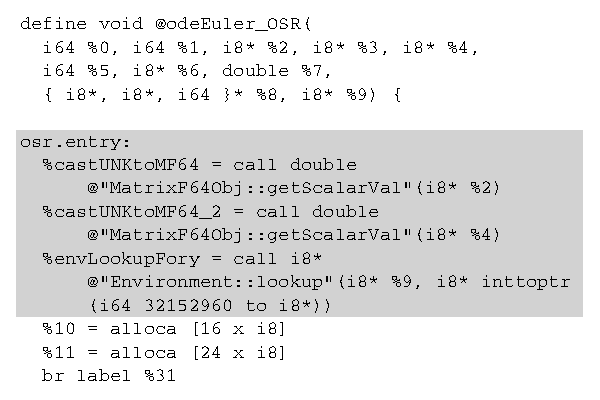
\includegraphics[width=0.9\columnwidth]{figures/comp-code/comp-code.eps}
\caption{\protect\label{fig:comp-code} Compensation code generated for {\tt odeEuler}. McVM instructions for unboxing variables to {\tt double} and fetching object {\tt y} from the environment are in grey. Two arrays of bytes are then allocated on the stack.
}
\end{center}
\end{figure}
\fi

%%%%%%%%%%%%%%%%%%%%%%%%%%%%%
\paragraph{Optimizer.}
The optimizer is called as {\tt gen} function in the open OSR stub (see \myfigure\ref{fi:overview-osr-open}) created by the OSR inserter. It receives the IR version \fIR\ of function \fbase, the basic block of \fIR\ where the OSR was fired, and the native code address of the \feval\ target function \gTarget. As a first step, the optimizer looks up the IR code of \gTarget\ by its address and checks whether a previously compiled version of \fBase\ specialized with \gTarget\ was previously cached.
%The core of our optimization pipeline is the optimizer module, which is responsible for generating optimized code for the running function \fBase\ using contextual information passed by an open-OSR stub. As a first step, the optimizer inspects {\tt val} to resolve the target $g$ of the \feval\ and checks whether a previously compiled version of \fBase\ optimized for $f$ is available from the cache.
\ifdefined \fullver
If not, a new function \fOptIIR\ is generated by cloning the IIR representation \fIIR\ of \fBase\ and by replacing all the \feval\ calls in the same group of the instrumented one with direct calls to \gTarget.
\else
If not, a new function \fOptIIR\ is generated by cloning the IIR representation \fIIR\ of \fBase\ and by replacing all \feval\ calls to \gTarget\ in \fOptIIR\ with direct calls.
\fi

\ifdefined \fullver
As a next step, the optimizer asks the IIR compiler to process \fOptIIR\ and generate optimized LLVM IR \fOptIR, also storing the variable map between IIR and IR objects when compiling the direct call corresponding to the \feval\ instruction that triggered the OSR.
This map is essential for the next step, which is constructing a state mapping between \fIR\ to \fOptIR, as it is compared against the corresponding map stored during the lowering of \fIIR\ to determine whether for each value in \fOptIR\ live at the continuation block:
\begin{itemize}[noitemsep, partopsep=0.5ex, topsep=0.5ex]
\item an {\tt llvm::Value*} from \fIR\ passed as argument at the OSR point can be used directly
\item or, compensation code is required to reconstruct its value before jumping to the block.
\end{itemize}
\else
As a next step, the optimizer asks the IIR compiler to lower \fOptIIR\ to \fOptIR. During the process, the compiler stores the variable map between IIR and IR objects at the direct call replacing the \feval\ instruction that triggered the OSR.

Using this map and the one stored during the lowering of \fIIR, the optimizer constructs a state mapping between \fIR\ and \fOptIR. In particular, for each value in \fOptIR\ live at the continuation block we determine whether we can assign to it a live value passed at the OSR point, or a compensation code is required to set its value.

Notice that, since the type inference engine yields more accurate results for \fOptIIR\ compared to \fIIR, the IIR compiler can in turn generate efficient specialized IR code for representing and manipulating IIR variables, and compensation code is typically required to unbox or downcast some of the live values passed at the OSR point.
\ifdefined \fullver
Compensation code might also be required to materialize an IR object for an IIR variable that were previously accessed through get/set methods from the environment. %TODO
\fi

\ifdefined \fullver
Once a state mapping object has been constructed, the optimizer calls our OSR library to generate the continuation function for the OSR transition and eventually compiles it.
A pointer to the compiled function is stored in the code cache and returned to the stub, which invokes it through an indirect call passing the live state saved at the OSR point.
\else
Once a state mapping has been constructed, the optimizer asks \osrkit\ to generate the continuation function for the OSR transition and then executes it.
\fi

An example of compensation code is reported in \myfigure\ref{fig:comp-code}. In order to correctly resume the execution at the first instruction in basic block {\tt \%31}, the entrypoint of {\tt odeEuler}'s continuation function executes a sequence of instructions that: 1) convert to {\tt double} two live variables -- i.e., function arguments {\tt \%2} and {\tt \%4} -- that are represented as boxed values in the unoptimized function, 2) look up in McVM's environment {\tt \%9} the pointer to the object instantiated for the symbol description stored at address {\tt 0x32152960}, and 3) allocate on the stack two buffers of 16 and 24 bytes, respectively.

%%%%%%%%%%%%%%%%%%%%%%%%%%%%%
\paragraph{Discussion.}
The ideas presented in this section advance the state of the art of \feval\ optimization in MATLAB runtimes.
%combine the flexibility of OSR-based specialization with the efficiency of the JIT-based method. 
Similarly to OSR-based specialization, we do not place restrictions on the functions that can be optimized. On the other hand, we work at IIR (rather than IR) level as in JIT-based specialization, which allows us to perform type inference on the code with direct calls. Working at IIR level eliminates the two main sources of inefficiency of OSR-based specialization: 1) we can replace generic instructions with specialized instructions, and 2) the types of $g$'s arguments do not need to be cached or guarded as they are statically inferred. These observations are confirmed in practice by experiments on benchmarks from the MATLAB community, as we will show in \mysection\ref{ss:experim-results}.